\documentclass[12pt,a4,twoside]{article}
\usepackage{polyglossia}
\usepackage[style=iso-numeric]{biblatex}
\usepackage[utf8]{inputenc}
\usepackage{amsmath}
\usepackage{graphicx}
\usepackage{float}
\usepackage[margin=2.5cm]{geometry}
\usepackage{hyperref}

\setmainlanguage{english}
\addbibresource{bib/ref.bib}

\def\abstract{
    \section*{\abstractname}
    \markboth{\MakeUppercase{\abstractname}}{}
}
\def\endabstract{\clearpage}

\providecommand{\keywords}[1]
{
  \small	
  \textbf{\textit{Keywords -- }} #1
}

\begin{document}

\begin{titlepage}

\newcommand{\HRule}{\rule{\linewidth}{0.1mm}}

\center
 
% ----------------------------------------------------------------------------------------
%	 HEADING SECTIONS
% ----------------------------------------------------------------------------------------


\includegraphics[scale=.75]{graphics/logo-fit-en-cerna.pdf}\\[2cm]
\textsc{\Large Information Security}\\[0.5cm]
\textsc{\large NI-IBE}\\[0.5cm]

% ----------------------------------------------------------------------------------------
%	 TITLE SECTION
% ----------------------------------------------------------------------------------------

\HRule \\[0.4cm]
{ \huge \bfseries Software Development Security}\\[0.4cm]
\HRule \\[1.5cm]
 
% ----------------------------------------------------------------------------------------
%	 AUTHOR SECTION
% ----------------------------------------------------------------------------------------

\begin{minipage}{0.4\textwidth}
\begin{flushleft} \large
\emph{Autor:}\\
Tomáš \textsc{PATRO}\\
\end{flushleft}

\end{minipage}\\[2cm]

% ----------------------------------------------------------------------------------------
%	 DATE SECTION
% ----------------------------------------------------------------------------------------

{\large \today}\\[2cm]

\vfill

\end{titlepage}

\newpage

\begin{abstract}

TODO ABSTRACT\\

\noindent
\keywords{todo1, todo2}
\end{abstract}

\tableofcontents
\newpage

\section*{Introduction}
\addcontentsline{toc}{section}{Introduction}

TODO

\newpage

\section{Software Development Life Cycle (SDLC)}
\label{sec:sdlc}

In this section, we talk about the software development life cycle. It is a fundamental term in software engineering, and it is good first to gain a better knowledge of this process, so we can put it into the context of the development security.

Every controlled process has some form of the life cycle, which determines the particular steps we take from the beginning to the end of the process. If we have a defined process, we can also define the resources and additional information connected to each step of the process. It is not different from the development of a piece of software.

The software development life cycle also defines several steps that determine the process of development of the software. These steps are the application of standard business practices to building software applications. The process is typically divided into six to eight steps. Some project managers may combine, split, or omit some steps, depending on the project's scope. \cite{sdlc_phoenix}

\begin{figure}[h]
\centering
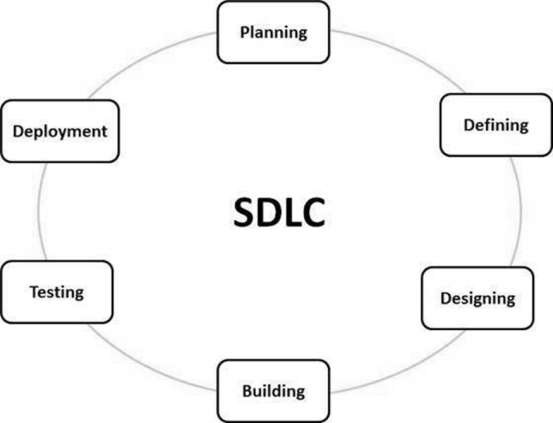
\includegraphics[width=.8\textwidth]{figures/sdlc_stages.jpg}
\caption{A typical SDLC consists of these stages \cite{sdlc_tutorials_point}}
\label{fig:sdlc_stages}
\end{figure}

\subsection{Planning}

Planning is often tightly connected with the requirements analysis. The senior team members often perform it. The inputs mostly come from the customer, sales department, market surveys, and domain experts in the industry. This information is later used to plan the project approach and conduct the feasibility study. \cite{sdlc_tutorials_point}

Another part of the planning may also be quality assurance requirements. These requirements often involve the identification of the risks associated with the project. The risks are often included in the feasibility study's technical part, which may also contain an overview of the security risks. \cite{sdlc_tutorials_point}

\subsection{Defining}

Once the requirements analysis is done, the next step is to clearly and formally document the product requirements, which are later discussed and approved by the customer or the market analysts. There is often a need to redefine these requirements based on customer feedback or feedback from other sources. The redefining can also be connected to the searching for potential security threads and risks. \cite{sdlc_tutorials_point}

\subsection{Designing}

The design involves the architects to come out with the best architecture for the product to be developed. The product of this step is often some form of a design specification. This specification is then reviewed by all important stakeholders and based on various parameters as risk assessment, product robustness, design modularity, etc. \cite{sdlc_tutorials_point}

Some aspects of the design include architecture, user interface, platforms, programming, and communications. The security aspect is also often a part of this step. It defines the measures to be taken to secure the application and can involve things like SSL encryption, password protection, and secure storage of user credentials. \cite{sdlc_phoenix}

\subsection{Building}

In this stage, the actual code is written, and the product is built. Developers must follow the coding guidelines defined by their organization, and programming tools like compilers, interpreters, debuggers, etc., are used to generate the code. The guidelines may include a set of best practices that often help write a better and more secure code. \cite{sdlc_tutorials_point}

The coding process also includes many other tasks. The developers often face tasks like finding and fixing errors and critical glitches. These aspects can often hold up the development process. However, it is also important for the code's overall security to address these issues in the development process. \cite{sdlc_phoenix}

Documentation can also be a guideline of the application's basic features. It can have a form of written documentation like user guides, troubleshooting guides, edge cases analysis, etc. \cite{sdlc_phoenix}

\subsection{Testing}

This step is often a subset of all the stages in the SDLC. However, this step refers to the testing only stage of the product where we detect products' security issues, bugs, glitches, and other types of defects. The defects need to be addressed and reprogrammed accordingly. This step should end only if the product reaches the company's quality standards. \cite{sdlc_tutorials_point}

Much of the testing can also be automated. This also includes security testing like static or dynamic code analysis, etc. \cite{sdlc_phoenix}

\subsection{Deployment}

The deployment involves a formal release of the product in the appropriate market. Sometimes the product deployment happens in stages as per the business strategy of the company. The product may be first released in a limited segment and tested in the real business environment (user acceptance testing). Based on the feedback, the product may be adjusted accordingly. There is also a space for finding potential bugs or security issues not detected by the testing phase. \cite{sdlc_tutorials_point}

Many companies prefer to automate the deployment phase. The automation may be complex and needs to be finely orchestrated not to bring security defects to the deployment process. \cite{sdlc_phoenix}

\subsection{Operation and Maintenance}

At this point, the product is developed and used in the field. However, the operation and maintenance phase is still important. In this step, the users discover and report bugs and security issues that weren't found during coding and testing. These errors need to be resolved, which may spawn new development cycles. \cite{sdlc_phoenix}

Often, a part of this phase is also some form of service-level agreement (SLA) between the customer and provider. This agreement documents what services the provider will furnish and defines the service standards the provider is obligated to meet. This may also include security measures that will be taken by the service provider are defined. Typically, this includes the drafting and consensus on antipoaching, IT security, and nondisclosure agreements. \cite{sla}

\subsection{SDLC Summary}

Based on the steps described above, we may conclude that development security is included in all the SDLC steps (phases). We can ask ourselves the question of how to approach security in the development process. There may be many answers to this question. One possible solution may be to define a set of standards/processes that should be followed throughout the SDLC.

\section{Secure Software Development Processes}

In this section, we look at the three processes which are used to ensure the security during the SDLC. The focus is put on three forefront representatives, namely Microsoft's \textit{Security Development Lifecycle} (SDL) \cite{microsoft_sdl}, OWASP’s \textit{Comprehensive, Lightweight Application Security Process} (CLASP) \cite{owasp}, and McGraw' \textit{Touchpoints} \cite{mcgraw2004software}.

In section \ref{sec:sdlc} we stated that the security issues are present in all phases of the SDLC. However, the construction of secure software is still largely a matter of guidelines, best practices, and undocumented expert knowledge in many companies. \cite{on_secure_software}

Several advances have been made in the definition of the process for secure software development by the major players in the field like Microsoft or OWASP. The information about the processes are taken from the \textit{Bart De Win's} paper \textit{On the secure software development process: CLASP, SDL and Touchpoints compared} \cite{on_secure_software}.

\subsection{Security Development Lifecycle}

In 2002, Microsoft made a commitment to follow the so-called ``trustworthy computing'' principle. As a result, the company defined the \textit{Security Development Lifecycle (SDL)}. SDL is a process definition that is composed of a set of activities, which complement Microsoft's development process. These activities are particularly aimed to address security issues during the development process. The following aspects characterize the process:

\begin{enumerate}
    \item Security as a supporting quality
    \item Well-defined process
    \item Good guidance
    \item Management perspective
\end{enumerate}

\subsubsection{Security as a Supporting Quality}



\subsubsection{Well-defined Process}

\subsubsection{Good Guidance}

\subsubsection{Management Perspective}











\newpage
\printbibliography

\end{document}
